\documentclass[aspectratio=169,dvipsnames]{beamer}
\usepackage{graphicx}
\usepackage{tikz}
\usetikzlibrary{shapes,arrows,positioning}
\usepackage[export]{adjustbox}
\usepackage[brazil]{babel}

\subtitle{Prof. Daniel C. Araújo}
\setbeamercolor{title page}{fg=RoyalBlue}
\setbeamercolor{date}{fg=OliveGreen}
\setbeamertemplate{title page}
{
  \vfill
  \begin{centering}
    {\usebeamerfont{title}\usebeamercolor[fg]{title}\inserttitle\par}
    \vskip0.25em%
    {\usebeamerfont{subtitle}\usebeamercolor[fg]{subtitle}\insertsubtitle\par}
    \vskip0.5em%
    %{\usebeamerfont{date}\usebeamercolor[fg]{date}\insertdate\par}
    \vfill
  \end{centering}
}


% Remove o rodapé
\setbeamertemplate{footline}{}

% Define o cabeçalho com os logos
\setbeamertemplate{headline}{
  \leavevmode%
  \begin{beamercolorbox}[wd=\paperwidth,ht=0.6cm,dp=0.5cm,right, colsep*=0pt]{section in head/foot}%
    
\includegraphics[height=0.8cm,valign=c]{Figs/Comum/unb.png} 
  \end{beamercolorbox}%
  \vskip0pt%
  \tikz \draw[thick] (0,0) -- (\paperwidth,0); % desenha a linha horizontal
}


\setbeamertemplate{footline}{
  \leavevmode%
    \tikz \draw[thick] (0,0) -- (\paperwidth,0);
  \hbox{%
  \begin{beamercolorbox}[wd=\paperwidth,ht=2.5ex,dp=3ex,center]{section in foot/foot}%
    Princípios de Comunicação para Engenharia
  \end{beamercolorbox}}%
  \vskip0pt%
}
% Remove os elementos padrão do cabeçalho
\title{Modulação FM}
\date{\today}


\begin{document}

\begin{frame}
  \titlepage
\end{frame}

\section{Receptor FM}

\begin{frame}{Modelo de Sinal recebido}

\begin{columns}[T] % alinhamento vertical no topo
    \begin{column}{0.5\textwidth} % define a primeira coluna
        
        \begin{block}{Caracterização do sinal de entrada}
            \begin{align*}
                u(t) &= A_c \cos[2\pi f_c t + \phi(t)], \\
                \phi(t) &= 2\pi k_f \int_{-\infty}^{t} m(\tau) d\tau.
            \end{align*}
        \end{block}

    \end{column}
    
    \begin{column}{0.5\textwidth} % define a segunda coluna

        \begin{figure}
            \centering
            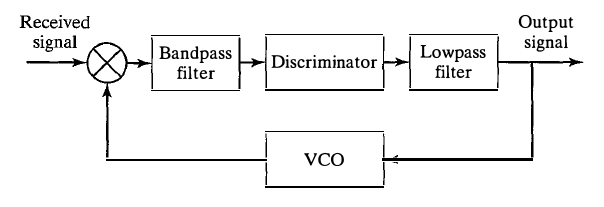
\includegraphics[width=\linewidth]{Figs/FM/PLL.png}
            \caption{Estrutura do PLL}
            \label{fig:enter-label}
        \end{figure}

    \end{column}
\end{columns}

\end{frame}


\begin{frame}{Modelo de Sinal do VCO}

\begin{columns}[T] % alinhamento vertical no topo
    \begin{column}{0.5\textwidth} % define a primeira coluna
        
        \begin{block}{Sinal do VCO}
            \begin{align*}
            y_v(t) &= A_v \sin[2\pi f_c t + \phi_v(t)], \\
            \phi_v(t) &= 2\pi k_v \int_{0}^{t} v(\tau) d\tau.
            \end{align*}
        \end{block}

    \end{column}
    
    \begin{column}{0.5\textwidth} % define a segunda coluna

        \begin{figure}
            \centering
            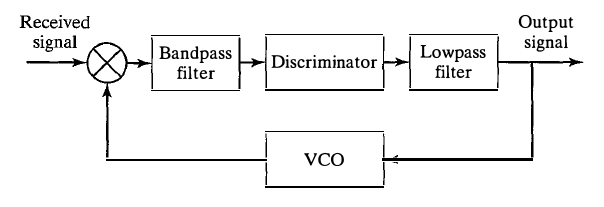
\includegraphics[width=\linewidth]{Figs/FM/PLL.png}
            \caption{Estrutura do PLL}
            \label{fig:enter-label}
        \end{figure}

    \end{column}
\end{columns}

\end{frame}


\begin{frame}{Comparador  de Fase}

         \begin{align*}
            y_v(t) &= A_v A_c\sin[2\pi f_c t + \phi_v(t)]\cos[2\pi f_c t + \phi(t)] * h(t), \\
            & \approx \frac{1}{2} A_vA_c \sin(\phi(t) - \phi_v(t))
            \end{align*}

\begin{figure}
            \centering
       \begin{tikzpicture}[auto, node distance=2cm,>=latex']

        % Nós
        \node [draw, circle] (mixer) {};
        \node [draw, rectangle, right of=mixer, node distance=2.5cm] (bandpass) {Bandpass filter};
        \node [draw, rectangle, right of=bandpass, node distance=2.5cm] (discriminator) {Discriminator};
        \node [draw, rectangle, below of=discriminator, node distance=2cm] (vco) {VCO};
        \node [draw, rectangle, right of=discriminator, node distance=2.5cm] (lowpass) {Lowpass filter};

        % Conexões
        \draw [->] (mixer) -- node[name=u] {} (bandpass);
        \draw [->] (bandpass) -- (discriminator);
        \draw [->] (discriminator) -- (lowpass);
        \draw [->] (lowpass) |- (vco);
        \draw [->] (vco) -| (mixer);

        % Entradas e saídas
        \draw [->] ([xshift=-1cm]mixer.west) -- (mixer) node[midway,above] {Received signal};
        \draw [->] (lowpass.east) -- ++(1.5,0) node[midway,above] {Output signal};

    \end{tikzpicture}
            \caption{Estrutura do PLL}
            \label{fig:enter-label}
        \end{figure}

 

\end{frame}




\end{document}
